%%%%%%%%%%%%%%%%%%%%%%%%%%%%%%%%%%%%%%%%%%%%%%%%%%%%%%%%%%%%%%%%%
% MUW Presentation
% LaTeX Template
% Version 1.0 (27/12/2016)
%
% License:
% CC BY-NC-SA 4.0 (http://creativecommons.org/licenses/by-nc-sa/3.0/)
%
% Created by:
% Nicolas Ballarini, CeMSIIS, Medical University of Vienna
% nicoballarini@gmail.com
% http://statistics.msi.meduniwien.ac.at/
%
% Customized for UAH by:
% David F. Barrero, Departamento de Automática, UAH
%%%%%%%%%%%%%%%%%%%%%%%%%%%%%%%%%%%%%%%%%%%%%%%%%%%%%%%%%%%%%%%%%

\documentclass[10pt,compress]{beamer} % Change 10pt to make fonts of a different size
\mode<presentation>

\usepackage[spanish]{babel}
\usepackage{fontspec}
\usepackage{tikz}
\usepackage{etoolbox}
\usepackage{xcolor}
\usepackage{xstring}
\usepackage{listings}

% Custom packages
\usepackage{hhline} % Confusion matrix
\usepackage{multicol}
\usepackage{multirow} % Confusion matrix
\usepackage{tikz}
\usepackage{pgfplots}
\def\layersep{2.5cm}
\usetikzlibrary{matrix,chains,positioning,decorations.pathreplacing,arrows,shapes}

\definecolor{dkgreen}{rgb}{0,0.6,0}
\definecolor{gray}{rgb}{0.5,0.5,0.5}
\definecolor{mauve}{rgb}{0.58,0,0.82}
 

\usetheme{UAH}
\usecolortheme{UAH}
\setbeamertemplate{navigation symbols}{} 
\setbeamertemplate{caption}[numbered]

%%%%%%%%%%%%%%%%%%%%%%%%%%%%%%%%%%%%%%%%%%%%%%%%%%%%%%%%%%%%%%%%%
%% Presentation Info
\title[Case Studies]{Case Studies}
\author{\asignatura\\\carrera}
\institute{}
\date{Departamento de Automática}
%%%%%%%%%%%%%%%%%%%%%%%%%%%%%%%%%%%%%%%%%%%%%%%%%%%%%%%%%%%%%%%%%


%%%%%%%%%%%%%%%%%%%%%%%%%%%%%%%%%%%%%%%%%%%%%%%%%%%%%%%%%%%%%%%%%
%% Descomentar para habilitar barra de navegación superior
\setNavigation
%%%%%%%%%%%%%%%%%%%%%%%%%%%%%%%%%%%%%%%%%%%%%%%%%%%%%%%%%%%%%%%%%

%%%%%%%%%%%%%%%%%%%%%%%%%%%%%%%%%%%%%%%%%%%%%%%%%%%%%%%%%%%%%%%%%
%% Configuración de logotipos en portada
%% Opacidad de los logotipos
\newcommand{\opacidad}{1}
%% Descomentar para habilitar logotipo en pié de página de portada
%\renewcommand{\logoUno}{Images/isg.png}
%% Descomentar para habilitar logotipo en pié de página de portada
%\renewcommand{\logoDos}{Images/CCLogo.png}
%% Descomentar para habilitar logotipo en pié de página de portada
\renewcommand{\logoTres}{Images/ALogo.png}
%% Descomentar para habilitar logotipo en pié de página de portada
%\renewcommand{\logoCuatro}{Images/ELogo.png}
%%%%%%%%%%%%%%%%%%%%%%%%%%%%%%%%%%%%%%%%%%%%%%%%%%%%%%%%%%%%%%%%%

%%%%%%%%%%%%%%%%%%%%%%%%%%%%%%%%%%%%%%%%%%%%%%%%%%%%%%%%%%%%%%%%%
%% FOOTLINE
%% Comment/Uncomment the following blocks to modify the footline
%% content in the body slides. 


%% Option A: Title and institute
\footlineA
%% Option B: Author and institute
%\footlineB
%% Option C: Title, Author and institute
%\footlineC
%%%%%%%%%%%%%%%%%%%%%%%%%%%%%%%%%%%%%%%%%%%%%%%%%%%%%%%%%%%%%%%%%


% This is for the confusion matrix, DELETE if not needed
\def\colorModel{hsb} %You can use rgb or hsb

\newcommand\ColCell[1]{
   \pgfmathparse{#1<50?1:0}  %Threshold for changing the font color into the cells
       \ifnum\pgfmathresult=0\relax\color{white}\fi
   \pgfmathsetmacro\compA{0}      %Component R or H
   \pgfmathsetmacro\compB{#1/100} %Component G or S
   \pgfmathsetmacro\compC{1}      %Component B or B
   \edef\x{\noexpand\centering\noexpand\cellcolor[\colorModel]{\compA,\compB,\compC}}\x #1
} 
%\newcolumntype{E}{>{\collectcell\ColCell}m{0.4cm}<{\endcollectcell}}  %Cell width
\newcommand*\rot{\rotatebox{90}}


\begin{document}

%%%%%%%%%%%%%%%%%%%%%%%%%%%%%%%%%%%%%%%%%%%%%%%%%%%%%%%%%%%%%%%%%
% Use this block for a blue title slide with modified footline
{\titlepageBlue
    \begin{frame}
        \titlepage
    \end{frame}
}

\institute{\asignatura}

\begin{frame}[plain]{}
   \begin{block}{Objectives}
      \begin{enumerate}
         \item Apply ML to realistic scenarios 
      \end{enumerate} 
   \end{block}

   \begin{block}{Bibliography}
	\begin{itemize}
%        \item Bishop, Christopher M. \textit{Pattern Recognition and Machine Learning}. 2nd edition. Springer-Verlag. 2011
        \item None
	\end{itemize}
   \end{block}
\end{frame}

{
\disableNavigation{white}
\begin{frame}[shrink]{Table of Contents}

 	\frametitle{Table of Contents}
  	\begin{multicols}{2}
  		\tableofcontents
    \end{multicols}

 %\frametitle{Table of Contents}
 %\tableofcontents
  % You might wish to add the option [pausesections]
\end{frame}
}

\section{Bank propensity model}
\begin{frame}{Case studies}{Case study 1: Bank propensity model}
	Client
	\begin{itemize}
		\item Bank
	\end{itemize}
	Business problem
	\begin{itemize}
		\item Identify those clients prone to buy a service
	\end{itemize}
	Data
	\begin{itemize}
		\item Available on several databases
		\item Historical data on service adquisition available
	\end{itemize}
	Propose a solution to:
	\begin{itemize}
		\item Data adquisition
		\item ML task
		\item Predictive or explicative model
		\item Model explotation
		\item Model maintenance
	\end{itemize}
\end{frame}

\section{Social media campaign impact}
\begin{frame}{Case studies}{Case study 2: Social media compaign impact}
	Client
	\begin{itemize}
		\item Car manufacturer
	\end{itemize}
	Business problem
	\begin{itemize}
		\item Real-time analysis of a campaign impact in Twitter
		\item Answer if people have a positive reaction to the campaign
	\end{itemize}
	Data
	\begin{itemize}
		\item None
	\end{itemize}
	Propose a solution to:
	\begin{itemize}
		\item Data adquisition
		\item ML task
		\item Predictive or explicative model
		\item Model explotation
		\item Model maintenance
	\end{itemize}
\end{frame}

\section{Hubble FGS-3 servo failure prediction}
\begin{frame}{Case studies}{Case study 3: Hubble FGS-3 servo failure prediction}
    \begin{columns}
 	   \column{.50\textwidth}
	   \small{
		Client
		\begin{itemize}
			\item NASA
		\end{itemize}
		Business problem
		\begin{itemize}
			\item Predict Hubble FGS-3 servo failure
		\end{itemize}
		Data
		\begin{itemize}
			\item Compensated error telemetry 
			\item Servo will fail if compensated error exceeds a threshold
		\end{itemize}
		Propose a solution to:
		\begin{itemize}
			\item ML task
			\item Predictive or explicative model
			\item Model explotation
			\item Model maintenance
		\end{itemize}
		}
 	   \column{.50\textwidth}
			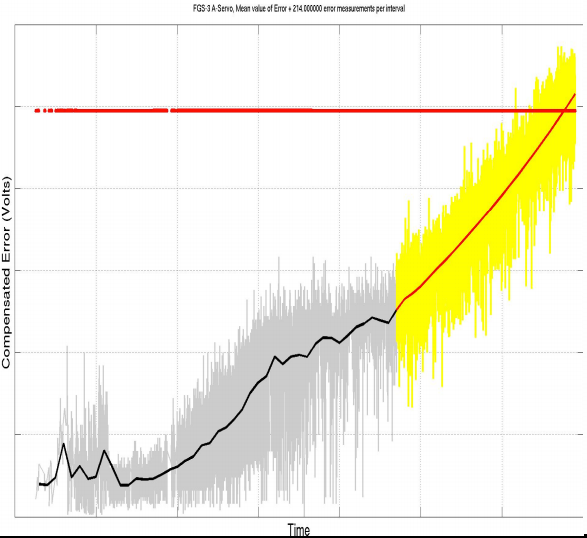
\includegraphics[width=\linewidth]{figs/hubble.png}

			\tiny \centering \href{https://ti.arc.nasa.gov/m/groups/machinelearningworkshop2017/MLW2017_slides/presentationsPDF/Hamed-Valizadegan.pdf}{(Source of this study case)}
    \end{columns}
\end{frame}

\section{Fall detection with accelerometer}
\begin{frame}{Case studies}{Case study 4: Fall detection with triaxial accelerometer}
    \begin{columns}
 	   \column{.50\textwidth}
	   \small{
		Client
		\begin{itemize}
			\item Technological start-up
		\end{itemize}
		Business problem
		\begin{itemize}
			\item Detect falls with a smartwatch
			\item Improve elderly people attention
		\end{itemize}
		Data
		\begin{itemize}
			\item None
		\end{itemize}
		Propose a solution to:
		\begin{itemize}
			\item Data adquisition
			\item ML task
			\item Data preprocessing
			\item Model explotation
			\item Model maintenance
		\end{itemize}
		}
 	   \column{.50\textwidth}
			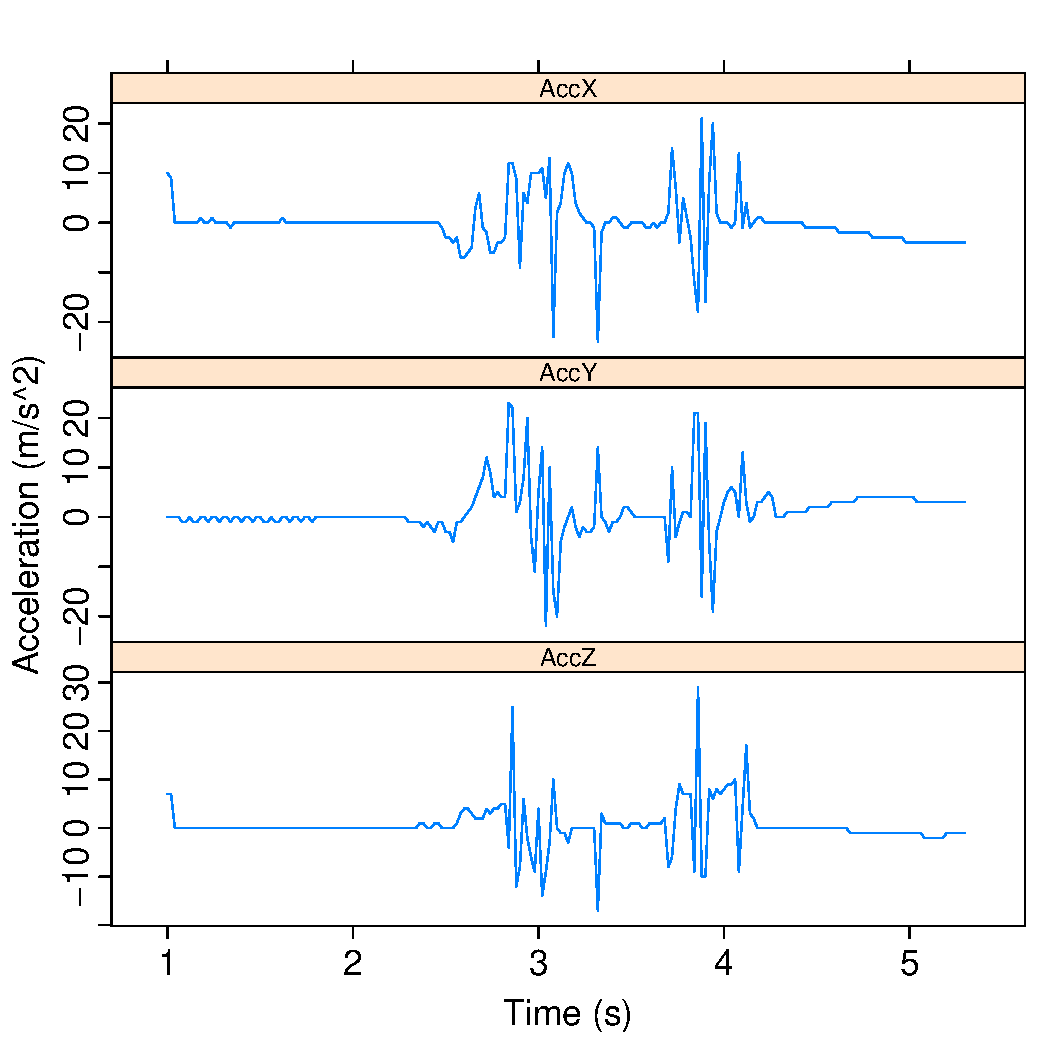
\includegraphics[width=\linewidth]{figs/HFall.pdf}

			\centering \href{https://www.slideshare.net/DavidFBarrero/triaxial-accelerometer-located-on-the-wrist-for-elderly-peoples-fall-detection}{(More info)}
    \end{columns}
\end{frame}

\section{Fall detection with sound}
\begin{frame}{Case studies}{Case study 5: Fall detection with sound}
    \begin{columns}
 	   \column{.50\textwidth}
	   \small{
		Client
		\begin{itemize}
			\item Technological start-up
		\end{itemize}
		Business problem
		\begin{itemize}
			\item Detect falls with sound
			\item Improve elderly people attention
		\end{itemize}
		Data
		\begin{itemize}
			\item None
		\end{itemize}
		Propose a solution to:
		\begin{itemize}
			\item Data adquisition
			\item ML task
			\item Data preprocessing
			\item Model explotation
			\item Model maintenance
		\end{itemize}
		}
 	   \column{.50\textwidth}
			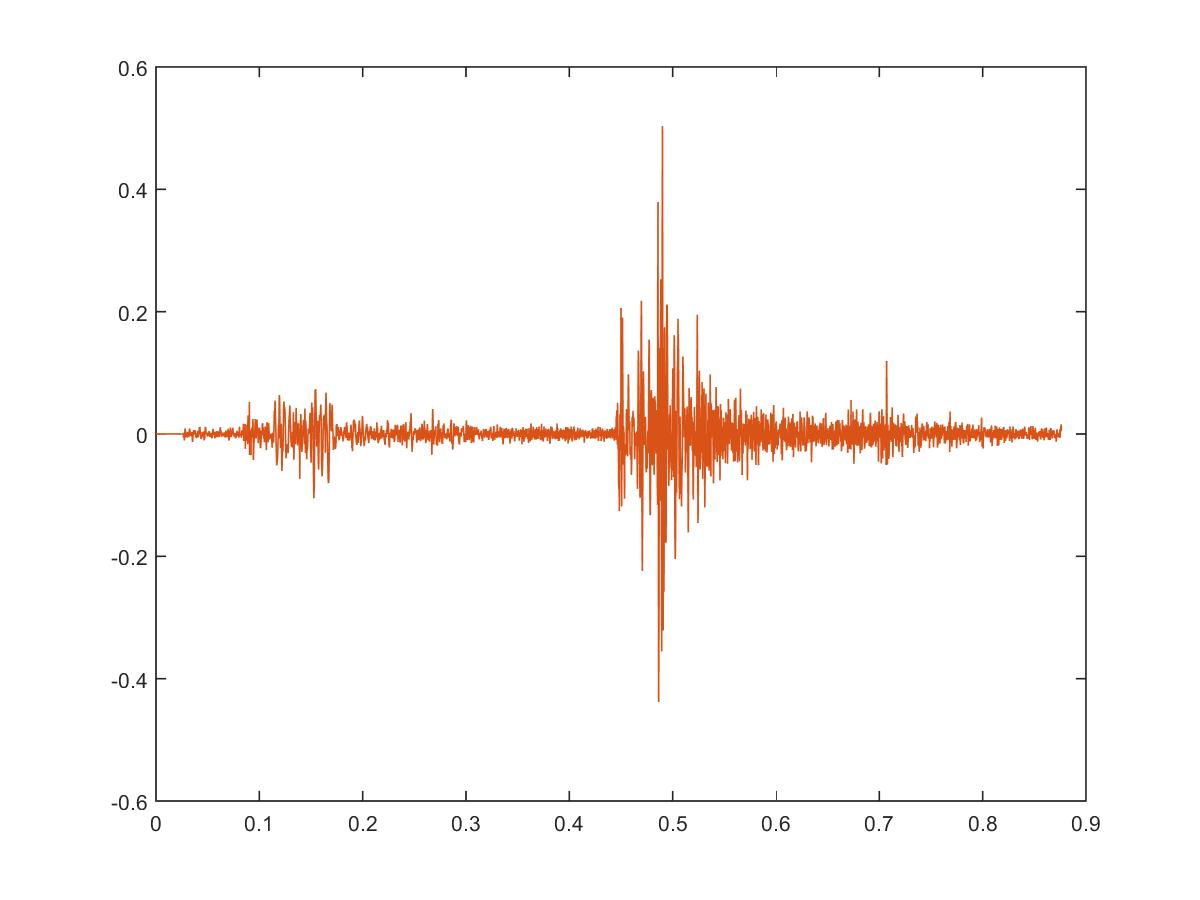
\includegraphics[width=\linewidth]{figs/sound.jpg}

			\footnotesize{
			\begin{tabular}{ll}
			\hline 
			Energy Mean & Energy Std \\
			Number of Zeros Mean & Number of Zeros Std \\
			Spectral Flux Mean & Spectral Flux Std \\
			Roll off Factor Mean & Roll off Factor Std \\
			Spectral centroid Mean & Spectral Centroid Std \\
			\hline
			\end{tabular} 
			}
			
			\centering \href{https://link.springer.com/chapter/10.1007/978-3-319-60042-0_18}{(More info)}
    \end{columns}
\end{frame}

\section{NASA JPL BioSleeve}
\begin{frame}{Case studies}{Case study 6: NASA JPL BioSleeve}
	\vspace{-0.5cm}
    \begin{columns}
	   \column{.50\textwidth}
	   \small{
		Client
		\begin{itemize}
			\item NASA JPL Advanced Robotics Group
		\end{itemize}
		Business problem
		\begin{itemize}
			\item Recognize hand gestures \href{https://spectrum.ieee.org/automaton/robotics/robotics-hardware/jpl-biosleeve-enables-precise-robot-control-through-hand-and-arm-gestures}{(more info)}
		\end{itemize}
		Data
		\begin{itemize}
			\item None
		\end{itemize}
		Propose a solution to:
		\begin{itemize}
            \item Data adquisition
			\item ML task
		\end{itemize}
		}

 	   \column{.50\textwidth}
			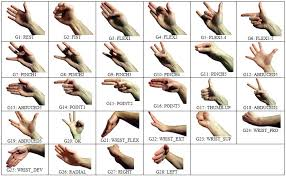
\includegraphics[width=\linewidth]{figs/biosleeve.jpeg}\\
			\tiny \centering \href{https://dces.essex.ac.uk/staff/hhu/Papers/CTS2013-San\%20Diego.pdf}{(Source)}

			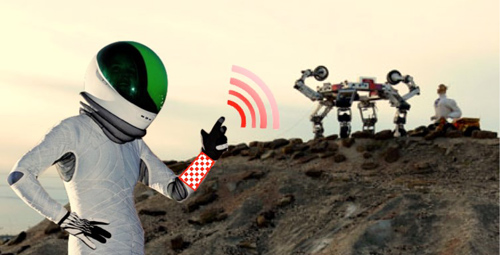
\includegraphics[width=0.5\linewidth]{figs/biosleeve2.jpg}\\
			\tiny \centering \href{https://www-robotics.jpl.nasa.gov/tasks/showBrowseImage.cfm?TaskID=277&tdaID=700081}{(Source)}
    \end{columns}

    \normalsize \href{https://dl.acm.org/citation.cfm?id=2447571}{Wolf, Michael T., et al. \textit{Decoding static and dynamic arm and hand gestures from the JPL BioSleeve}. IEEE Aerospace Conference. IEEE, 2013.}\\

	\vspace{0.3cm}

    \centering \href{https://www.semanticscholar.org/paper/JPL-BioSleeve-for-gesture-based-control\%3A-Technology-Assad-Wolf/18152a964e128e247a706dc8729036369b536b48/figure/2}{(Solution)} \href{https://www.youtube.com/watch?v=BGfDyqAE86U}{(Results)}
\end{frame}

\section{UAV terrain classification}
\begin{frame}{Case studies}{Case study 7: UAV terrain classification}
		Client
		\begin{itemize}
			\item NASA JPL Advanced Robotics Group
		\end{itemize}
		Business problem
		\begin{itemize}
			\item Recognize terrain type for automatic UAV landing
			\item \href{https://www.youtube.com/watch?v=ovtpwxiIr_8}{(Video)}
		\end{itemize}
		Data
		\begin{itemize}
			\item UAV down-looking camera
			\item No dataset available
		\end{itemize}
		Propose a solution to:
		\begin{itemize}
			\item Data adquisition
			\item ML task
            \item Feature extraction
		\end{itemize}
\end{frame}

\end{document}
